\documentclass[12pt]{article}  \usepackage{algorithm2e} \usepackage{amsmath} \usepackage{amsthm} \usepackage{amsfonts} \usepackage{bbm} \usepackage{color,soul} \usepackage{framed} \usepackage[margin=0.5in]{geometry} \usepackage{hyperref} \usepackage{mathtools}
\usepackage[dvipsnames]{xcolor}
\usepackage{tikz}  \newtheorem{theorem}{Theorem}[section] \newtheorem{lemma}[theorem]{Lemma} \newtheorem{proposition}[theorem]{Proposition} \newtheorem{corollary}[theorem]{Corollary}  \DeclarePairedDelimiter{\ceil}{\lceil}{\rceil} \DeclarePairedDelimiter{\floor}{\lfloor}{\rfloor} \DeclareMathOperator*{\argmin}{arg\,min} \DeclareMathOperator*{\argmax}{arg\,max} \newcommand{\D}{\mathrm{d}} \SetKwInput{KwInput}{Input} \SetKwInput{KwOutput}{Output}  \begin{document}
\section{Logistic Regression}\vspace{.1pt} \hrule height 2pt \smallskip \renewcommand{\arraystretch}{1}% Tighter \begin{description} \item[Intro] 
This model assumes that the log odds-ratio can be fit by a linear model. We start with the probability mass function for a \href{https://en.wikipedia.org/wiki/Bernoulli_distribution}{Bernoulli trial}: $f(y;p) = p^y \times (1-p)^{(1-y)}$ for $y \in \{0, 1\}$. We are interested in estimating what $p$ is, and so it's natural to conceive of a maximum likelihood estimator; since $\log$ monotone we can apply this transformation without changing the maximizer. The log-likelihood is given by $y \log p + (1-y) \log (1-p)$ using \href{https://en.wikipedia.org/wiki/Logarithm#Logarithmic_identities}{properties of logarithms}. In optimization, we generally work to minimize objective functions, and so it's then natural to set our (objective) \emph{loss function}
to be $- \left[y \log p + (1-y) \log (1-p)\right]$. In summary, we 
have, for $\sigma(x) = \frac{1}{1 + \exp(-x)}$:
\begin{align}
  z &= w^Tx + b \\
  \hat y &= a = \sigma(z) \\
  \mathcal{L}(a, y) &= - \left[y \log (a) + (1-y) \log (1-a)\right] \end{align}

We can draw a \emph{computation graph} to describe the forward pass as follows:
\begin{center}
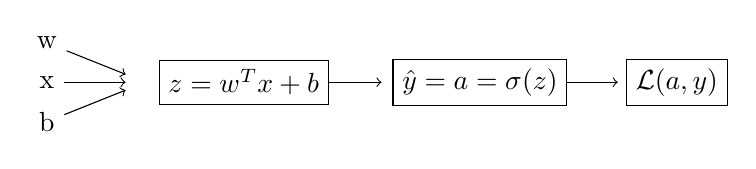
\begin{tikzpicture}   \node (w) at (0, 1) {w};
  \node (x) at (0, .5) {x};
  \node (b) at (0,0) {b};
  \draw[->] (w) to (1, .6);
  \draw[->] (x) to (1, .5);
  \draw[->] (b) to (1, .4);
  \node[draw=black,rectangle] (z) at (2.5, .5) {$z = w^Tx + b$};
  \draw[->] (z) to (4.25, .5);
  \node[draw=black,rectangle] (yhat) at (5.5, .5) {$\hat y = a = \sigma(z)$};
  \draw[->] (yhat) to (7.25, .5);
  \node[draw=black,rectangle] (loss) at (8, .5) {$\mathcal L (a,y)$};
\end{tikzpicture}
\end{center} We seek to learn $w, b$ to minimize the loss function. \emph{Back propogation} proceeds as follows:
\begin{align*}
\texttt{da} &= \frac{\partial \mathcal L}{\partial a} = - \left(\frac{y}{a} - \frac{1-y}{1-a}\right) = \frac{-y}{a} + \frac{1-y}{1-a}. \\
  \texttt{dz} &= \frac{\partial \mathcal L}{\partial z} = \frac{\partial \mathcal L}{\partial a}\frac{\partial a}{\partial z} = \left(\frac{-y}{a} + \frac{1-y}{1-a}\right) \times a(1-a) = \frac{-y}{a} \cdot a(1-a) + \frac{1-y}{1-a} \cdot (1-a) a = -y(1-a)+ (1-y)a \\ &= ay - y + a - ay = a - y.  \\
\texttt{dw} &= \frac{\partial \mathcal L}{\partial w} \overset{?}{=} \frac{\partial \mathcal L}{\partial z} \frac{\partial z}{\partial w} = (a-y) x^T. \\
\texttt{db} &= \frac{\partial \mathcal L}{\partial b} = \frac{\partial \mathcal L}{\partial z} \underbrace{\frac{\partial z}{\partial b}}_{=1}. \end{align*}
Our update rule then becomes: $w := w - \alpha \texttt{dw}$, and $b := b - \alpha \texttt{db}$. Our (average) \emph{cost} function is defined as $J(w,b) = \frac{1}{m} \sum_{i=1}^m \mathcal L(a^{(i)}, y^{(i)})$. Since $\frac{\partial}{\partial \cdot}$ is a linear operator, obtaining gradients is quite straightforward since we are left with a series of derivatives of loss functions, which we calculated above.
\begin{align*}    \frac{\partial J}{\partial w} = \frac{1}{m} \sum \frac{\partial \mathcal L}{\partial w}, \hspace{15pt} \textrm{and} \hspace{15pt} \frac{\partial J}{\partial b} = \frac{1}{m} \sum \frac{\partial \mathcal L}{\partial b} \end{align*}
Our optimization routine then becomes
\begin{algorithm}   \For{\texttt{i in range(m)}} {
    $z^{(i)} = w^Tx^{(i)} + b$ \\
    $a^{(i)} = \sigma(z^{(i)})$ \\
    $J += - \left[ y^{(i)} \log a^{(i)} + (1-y^{(i)}) \log (1 - a^{(i)}) \right]$ \\
    $\partial d z^{(i)} = a^{(i)} - y^{(i)}$ \\
    $\partial d w += \partial d z^{(i)} {x^{(i)}}^T$ \\
    $\partial d b += \partial d z^{(i)}$
}
$J /= m$ \\
$\partial w /= m$ \\
$\partial b /= m$ \end{algorithm}
The above concludes one round of \href{https://en.wikipedia.org/wiki/Gradient_descent}{Gradient Descent}. We repeat this procedure many times until training loss (and ideally test loss ) is sufficiently minimized. We remark that it's possible to remove both \texttt{for} loops (over the training data, and over the parameters in $w$) by using vectorized operations in \texttt{numpy}. We execute this in code \href{https://github.com/asantucci/NN/blob/master/logistic_regression.py#L46}{here}. \end{document}